\newpage
\section{High Entropy Token Ratio }

\autoref{fig:high_entropy_ratio} shows the ratio of high-entropy tokens measured on rollouts generated by the student model during \method~training, where entropy is computed from the teacher model. High-entropy tokens are defined as token positions whose teacher entropy exceeds a threshold $\tau$ $(=0.8)$, indicating regions where the teacher exhibits higher uncertainty.

As shown in the figure, the proportion of high-entropy tokens is relatively high during the early stages of training and decreases as training progresses. After convergence, the ratio stabilizes at approximately 15\% to 20\%. This observation motivates the random forward KL setting in~\S\ref{sec:fkl_placement}, where forward KL is applied to a randomly selected 20\% of token positions. In this setting, the ratio of tokens receiving forward KL is matched to \method, while the token selection is independent of the teacher’s uncertainty, serving as a controlled baseline.


\begin{figure}[H]
  \centering
    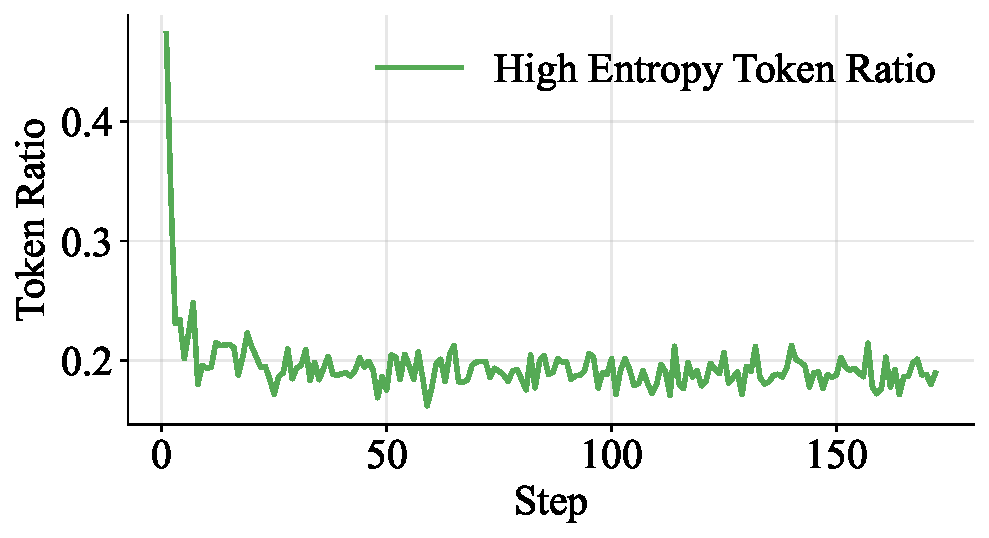
\includegraphics[width=0.5\linewidth]{figure/ratio_curve.pdf}
  \caption{Ratio of tokens with high teacher entropy in rollouts produced by the student model during \method~training.}
  \label{fig:high_entropy_ratio}
\end{figure}